\documentclass[addpoints,11pt]{exam}

\usepackage{alltt}
\usepackage[margin=1in]{geometry}   % set up margins
\usepackage[T1]{fontenc}
\usepackage[usenames,dvipsnames]{xcolor}
\usepackage{enumerate}              % fancy enumerate
\usepackage{amsmath}                % used for \eqref{} in this document
\usepackage{amsthm}
\theoremstyle{definition}
\newtheorem{exmp}{Example}[section]
\usepackage{verbatim}               % useful for \begin{comment} and \end{comment}
\usepackage{eurosym}                % used for euro symbol
\usepackage{caption} 
\usepackage{graphicx}
\graphicspath{{Figures/}}
\usepackage{subcaption}
\usepackage{color}
\usepackage{float}
\usepackage{amssymb}
\usepackage{sgamevar}
\usepackage{sgame}
\usepackage[colorlinks=true]{hyperref}
\hypersetup{colorlinks=true, citecolor=ForestGreen, linkcolor=BlueViolet, urlcolor=Magenta}

%Solutions or nah (blank next two lines out for no solutions, unblank #3)
%\printanswers
%\newcommand{\dd}[1]{\par {\textbf{\textcolor{red}{#1}}}}
\newcommand{\dd}[1]{}  


\setlength\parindent{0pt}
\unframedsolutions
\SolutionEmphasis{\color{red}}
\CorrectChoiceEmphasis{\color{red}}
\renewcommand{\choicelabel}{(\alph{choice})}
\newcommand{\blank}[0]{\underline{\hspace{3cm}}}
\pointformat{\bfseries[\thepoints]}
\pointpoints{pt}{pts}
\pointsinrightmargin




\begin{document}


\title{\textbf{Exam 2} \dd{Solutions} \\ \vspace{2 mm} {\large ECON 101}}
\author{Summer I 2016}
\date{}
\maketitle

\makebox[\textwidth]{Name:\enspace\hrulefill}
\\

\makebox[\textwidth]{ONYEN:\enspace\hrulefill}
\\

\makebox[\textwidth]{PID:\enspace\hrulefill}
\\

\makebox[\textwidth]{Honor Code Signature:\enspace\hrulefill}

\begin{center}
	\fbox{\fbox{\parbox{5.5in}{\centering
				This exam consists of 30 multiple choice questions and 2 short answer questions. Multiple choice questions should be bubbled in on a scantron. Extra paper for scratch work is attached. The total number of points available on this exam is \textbf{100}.}}}
\end{center}

\section*{Multiple Choice [2.5 pts each]}

Choose the option that best answers the question given.

\begin{questions}
	
\question When workers lose their jobs and become officially unemployed, the labor force participation rate

\begin{choices}
	\CorrectChoice remains constant.
	\choice increases. 
	\choice decreases.
	\choice Any of the above could occur.
\end{choices}

\begin{solution} 
	LFPR = (\#E + \#U)/(Adult pop.). All that occurs is a movement of workers from E to U, and so the LFPR does not change.
\end{solution}
	
\question A family in Ireland purchases leather loafers from an Italian shoe maker in Rome. As a result of this transaction, GDP in Ireland \blank and GDP in Italy \blank. 
		
		\begin{choices}
			\choice increases; remains unchanged
			\choice remains unchanged; decreases
			\CorrectChoice remains unchanged; increases
			\choice decreases; increases
			\choice None of the above
		\end{choices}
		
\begin{solution} 
	Ireland: $C$ increaeses, $NX$ falls by the same amount - GDP unchanged. Italy: $NX$ increases, GDP increases.
\end{solution}

\newpage

	\question Productivity is defined as 
	
	\begin{choices}
		\choice the stock of equipment and structures that are used to produce goods and services.
		\CorrectChoice the quantity of goods and services produced from each unit of labor input.
		\choice the inputs into the production of goods and services that are provided by nature.
		\choice the ``rules of the game'' that shape social interactions and structure economic incentives.
	\end{choices}
	
	\begin{solution} 
		See class notes.
	\end{solution}
	
	\question Suppose your grandma gives you \$1,000 in cash for your birthday. If you deposit the entire \$1,000 in your bank, what is the total potential increase in the money supply if the reserve requirement for banks is 20\%?
	
	\begin{choices}
		\choice \$0
		\choice \$1,000
		\choice \$5,000
		\CorrectChoice \$4,000
	\end{choices}
	
	\begin{solution} 
		Money multiplier: 1/.20 = 5. Potential increase in MS = \$1,000 $\times$ 5 = \$5,000 - \$1,000 (adds \$5,000 to deposits, took out \$1,000 in cash).
	\end{solution}
		


\question Which of the following is NOT a tool the Fed uses to influence the money supply?

\begin{choices}
	\CorrectChoice Raise/lower taxes
	\item Purchase/sell bonds
	\item Pay interest on reserves
	\item Set reserve requirements
	\item None of the above
\end{choices}

\begin{solution} 
	See class notes.	
\end{solution}	

		
\question Suppose an economy experienced a positive rate of inflation between 2003 and 2004 and again between 2004 and 2005. However, the inflation rate was lower between 2004 and 2005 than it was between 2003 and 2004. Which of the following is consistent with this scenario?
	
	\begin{choices}
		\choice The CPI was 100 in 2003, 110 in 2004, and 105 in 2005.
		\choice The CPI was 110 in 2003, 106 in 2004, and 100 in 2005.
		\CorrectChoice The CPI was 100 in 2003, 120 in 2004, and 135 in 2005.
		\choice All of the above are correct.
		\choice None of the above are correct.
	\end{choices}
	
\begin{solution} 
	If there was a positive rate of inflation from year-to-year, then the CPI should be increasing from 2003 to 2005. (c) is the only one for which this holds true, so only have to check that option. $\pi_{2004} = (120-100)/100 = 20\%$, $\pi_{2005} = (135-120)/120 = 12.5\%$.
\end{solution}


\question The quantity theory of money concludes that an increase in the money supply causes

\begin{choices}
	\choice a proportional increase in velocity.
	\choice a proportional increase in real output.
	\choice a proportional decrease in velocity.
	\CorrectChoice a proportional increase in prices.
	\choice a proportional decrease in prices.
\end{choices}

\begin{solution} 
	The Quantity Theory states that money is neutral and so increases in the money supply will be lead to a proportional increase in prices.
\end{solution}

\newpage	
	
\question A country has an annual growth rate of real GDP per capita of 2.5\%. Real GDP per capita in 2016 is \$20,000. Real GDP per capita in the country will be at least \$40,000 by
	
		\begin{choices}
			\item 2040.
			\CorrectChoice 2045.
			\item 2030.
			\item 2035.
		\end{choices}
		
	\begin{solution} 
		Doubling time: 70/2.5 = 28 years. Real GDP per capita will be double in 2044.
	\end{solution}
	

	
\question Continued long-run economic growth requires that economies
		
		\begin{choices}
			\choice continue to increase their savings rates.
			\choice reach their steady-state levels of capital and output.
			\choice have high levels of capital stock.
			\CorrectChoice have institutions in place that encourage development of new ideas.
		\end{choices}
		
		\begin{solution} 
			See class notes. Sustained long-run growth is due to technology.
		\end{solution}

	\question Figure \ref{MC22} shows the production function of a small country, as well as its investment and depreciation functions. Assume there is no population growth and the country is currently at its steady state.
	
	
	\begin{figure}[H]
		\centering
		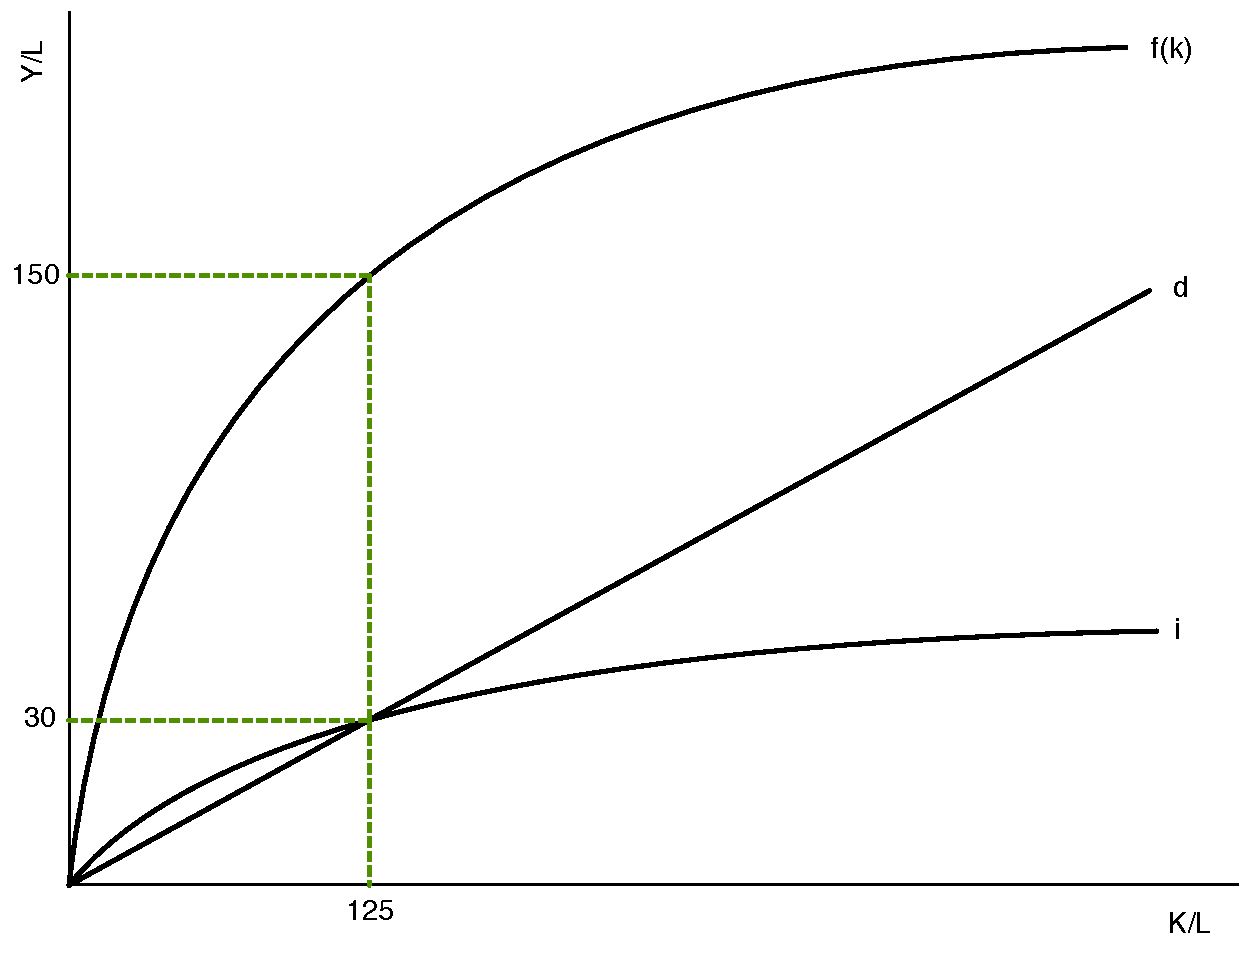
\includegraphics[scale=.35]{Final_MC22.pdf}
		\caption{Production, Investment, and Depreciation}
		\label{MC22}
	\end{figure}
	
	The percent of output per worker that is invested every period is \blank and the rate of capital depreciation is \blank.
	
	\begin{choices}
		\item 20\%; 20\%
		\CorrectChoice 20\%; 24\%
		\item 24\%; 20\%
		\item 24\%; 24\%
	\end{choices}
	
	\begin{solution} 
		$i^* = 30 = sy^* = s150 \Rightarrow s = 30/150 = 20\%$. $i^* = d^* = 30 = \delta k^* \Rightarrow \delta = 30/125 = 24\%$.
	\end{solution}
	
\newpage
	
	\question If there is an increase in the price of blueberries that causes consumers to purchase fewer pounds of blueberries and more pounds of strawberries, the CPI will suffer from
	
	\begin{choices}
		\choice bias due to the introduction of new goods.
		\choice bias due to unmeasured quantity change.
		\CorrectChoice substitution bias.
		\choice base-year bias.
		\choice none of the above.
	\end{choices}
	
	\begin{solution} 
		See class notes. Substitution from more expensive to cheaper goods biases the CPI.
	\end{solution}
	
\question Refer to Table \ref{tab3}. 
		
		\begin{table}[H]
			\centering
			\caption{Production in Utopia}
			\label{tab3}
			\begin{tabular}{c|c|c}        
				
				$k$ & $y$ & $MP_k$ \\
				\hline
				1000 & 100 & --- \\
				1001 & $x$ & $z$ \\
				1002 & $y$ & 5 \\
			
			\end{tabular}
		\end{table}
		
		Under the assumptions of production functions in the Solow model, which of the following holds true?
		
		\begin{choices}
				\choice $x>y$ and $z>5$
				\choice $x<y$ and $z<5$
				\choice $x>y$ and $z<5$
				\CorrectChoice $x<y$ and $z>5$
				\choice Impossible to know without more information.
		\end{choices}
		
	\begin{solution} 
		Higher levels of capital leads to greater output, so $x<y$. Diminishing marginal returns implies $z>5$.
	\end{solution}
	
	\question Savings is 
	
	\begin{choices}
		\choice the purchase of new capital goods.
		\choice the purchase of new consumption goods.
		\CorrectChoice income that is not spent on consumption goods.
		\choice income that is not spent on capital goods.
	\end{choices}
	
	\begin{solution}
		 See class notes.
	\end{solution}
	
	\question Suppose the money supply in an economy grows at 5\% and real output growth is 2\%. If velocity is constant, prices should rise by 
	
	\begin{choices}
		\choice exactly 5\%.
		\choice more than 5\% but less than 7\%.
		\CorrectChoice less than 5\%.
		\choice greater than 7\%.
	\end{choices}
	
	\begin{solution} 
		$\vec{M} + \vec{v} = \vec{Y} + \pi \Rightarrow 5\% + 0\% = 2\% + \pi \Rightarrow \pi = 3\%$.
	\end{solution}
	
\newpage
	
	\question How many of the following transactions would affect the consumption component of GDP?
	
	\begin{enumerate}[(i)]
		\item A family buys a new refrigerator.
		\item Jane purchases a used bookshelf from a friend.
		\item Your parents buy a bottle of Italian wine.
		\item A newly-wed couple buys a home.
	\end{enumerate}
	
	\begin{choices}
		\choice 0
		\choice 1
		\CorrectChoice 2
		\choice 3
		\choice 4
	\end{choices}	
	
	\begin{solution}
		 (i) and(iii) would be included in consumption. (ii) is not included because it is a used good, an (iv) is included in investment.
	\end{solution}
	
	\question A company is planning to finance the construction of a new factory, but has limited funds. In order to procure the necessary funds, the company is likely to 
	
		\begin{choices}
			\choice demand loanable funds by buying bonds.
			\choice supply loanable funds by selling bonds.
			\choice supply loanable funds by buying bonds.
			\CorrectChoice demand loanable funds by selling bonds.
		\end{choices}
		
		\begin{solution} 
			The company would demand loanable funds. Borrows money by selling bonds.
		\end{solution}
		
	\question Figure \ref{MC27} shows the market for loanable funds. 

	
	\begin{figure}[H]
		\centering
		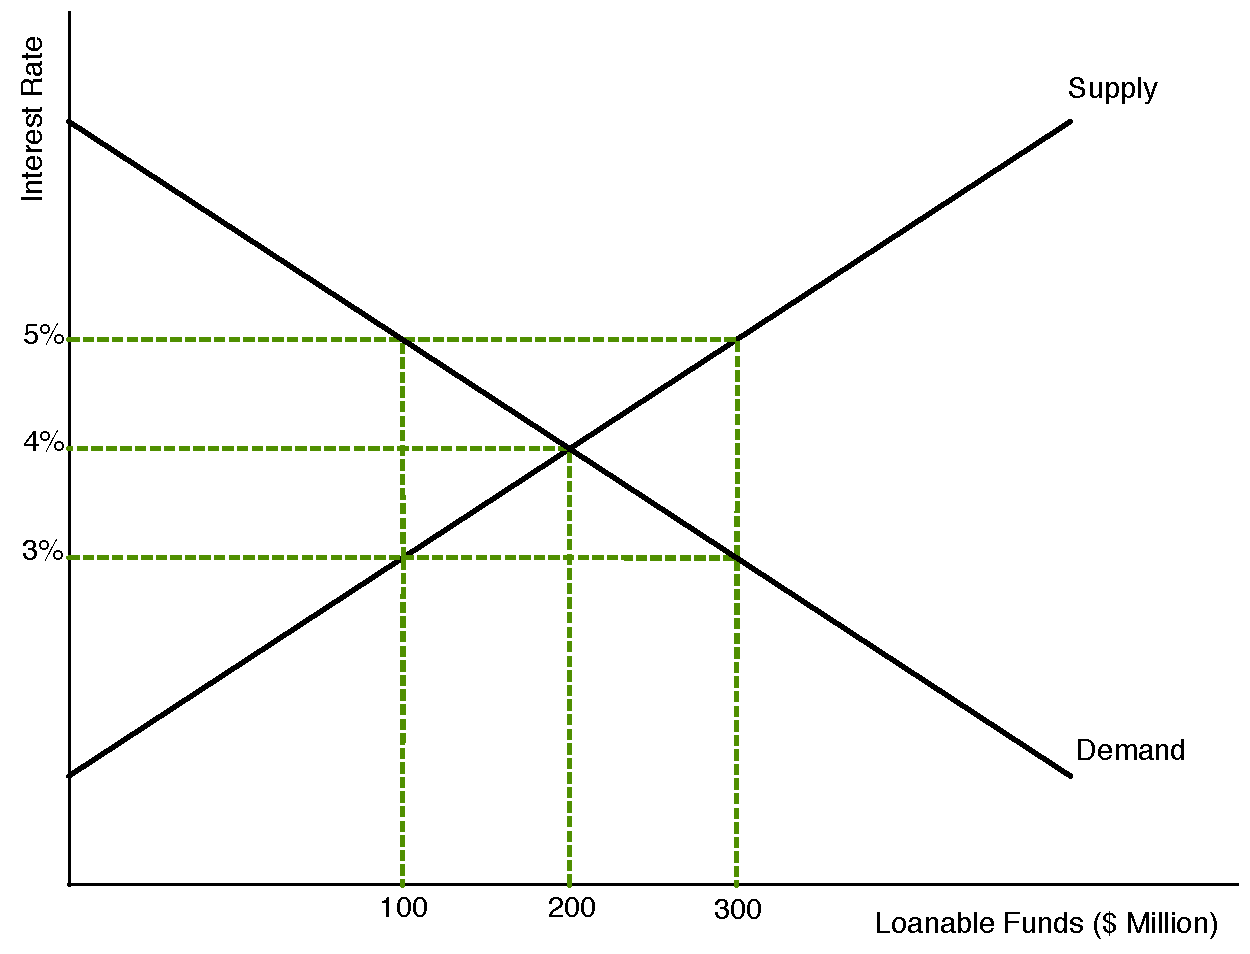
\includegraphics[scale=.38]{Exam2_MC27.pdf}
		\caption{Market for Loanable Funds}
		\label{MC27}
	\end{figure}

	If the interest rate in the market is 3\%, then 
	
	\begin{choices}
		\choice investment exceeds savings by \$300 million.
		\choice investment exceeds savings by \$200 million.
		\CorrectChoice borrowing demands exceed savings by \$200 million.
		\choice borrowing demands exceed savings by \$300 million.
	\end{choices}
	
	\begin{solution}
		 At an interest rate of 3\%, borrowing demand exceeds savings and thus there is a shortage of loanable funds of \$200 million.
	\end{solution}
	
\newpage
	
	\question Suppose you lend your roommate \$100 for one year at 8\% nominal interest. You both expect the real interest rate on the loan to be 10\%. If at the end of the loan wealth was transferred from your roommate to you, then actual inflation over the course of the year could have been
		
		\begin{choices}
			\CorrectChoice $-4\%$.
			\choice $3\%$.
			\choice $9\%$.
			\choice $-1\%$.
			\choice None of the above.
		\end{choices}
		
		\begin{solution}
			 $r^* = i - \pi^e \Rightarrow \pi^e = i - r^* = -2\%$. If wealth is transferred from your roommate (borrower) to you (lender), then $\pi < \pi^e$ and so $\pi < -2\%$.
		\end{solution}
	
	
	\question In 2014, an economy produced 100 apples that are sold for \$1.50 each and 125 oranges for \$2 each. The next year, the economy again produced 100 apples, but for \$1.25 each, and 140 oranges for \$2.25. Using 2014 as the base year, the GDP deflator in 2014 is \blank, while the GDP deflator in 2015 is \blank.
	
	\begin{choices}
		\choice 98; 100
		\choice 102; 100
		\CorrectChoice 100; 102
		\choice 100; 98
		\choice None of the above.
	\end{choices}
	
	\begin{solution} 
		Since the base year is 2014, GDP deflator in 2014 is 100. In 2015, nominal GDP = $100(\$1.25) + 140(\$2.25) = \$440$ (current quantity and prices). Real GDP in 2015 = $100(\$1.50) + 140(\$2.00) = \$430$ (current quantity, base year prices). GDP deflator in 2015 = $(440)/(430)\times 100 = 102.3$.
	\end{solution}	
	

	
	
	\question In the presence of an investment tax credit, how many of the following are FALSE?
	
		\begin{enumerate}[(i)]
			\item The real interest rate will increase.
			\item The quantity of investment will decrease.
			\item The quantity of savings will increase.
		\end{enumerate}
		
		\begin{choices}
			\choice 0
			\CorrectChoice 1
			\choice 2
			\choice 3
		\end{choices}	
	
	\begin{solution} 
		An investment tax credit will increase the demand for loanable funds. As a result, the real interest rate and both savings and investment will increase.
	\end{solution}

	
	\question \textit{The New York Times} cost \$0.15 in 1970 and \$0.75 in 2000. If average wages in the US were \$3.23 per hour in 1970 and \$14.32 in 2000, then the purchasing power of workers in terms of newspapers 
	
	\begin{choices}
		\CorrectChoice was greater in 1970 than in 2000.
		\choice was greater in 2000 than in 1970.
		\choice was equal in 1970 and 2000.
		\choice impossible to discern without more information.
	\end{choices}
	
	\begin{solution}
		 Workers in 1970 could purchase $3.23/.15 = 21.5$ newspapers for every hour they worked, while workers in 2000 could only purchase $14.32/.75 = 19.09$ newspapers for each hour worked.
	\end{solution}
	
\newpage

\question Jonathan takes \$500 of currency from her wallet and deposits it in a checking account. If the bank adds the entire \$500 to reserves, the money supply \blank, but if the bank lends out some of the \$500, the money supply \blank.

\begin{choices}
	\choice increases; increases even more
	\choice increases; increases by less
	\CorrectChoice is unchanged; increases
	\choice decreases; decreases by less
\end{choices}

\begin{solution} 
	If the bank holds all deposits as reserves, no money is created. Money is created in a fractional reserve system.
\end{solution}

	
\question A bag of sugar is sold to Coca Cola for \$0.50, which uses this sugar to make Sprite that is sold to consumers for \$1.25. Another bag of of sugar is sold to Food Lion for \$1.25, where it is sold to consumers for \$2.75. Together, these transactions have what effect on GDP?

\begin{choices}
	\choice Increase GDP by \$1.75
	\CorrectChoice Increase GDP by \$4.00
	\choice Increase GDP by \$5.75
	\choice Increase GDP by \$3.00
\end{choices}

\begin{solution} 
	Only the sale of final goods is included in GDP: \$1.25 + \$2.75 = \$4.
\end{solution}
	
	\question Which of the following policy combinations would consistently work to increase the money supply?
	
	\begin{choices}
		\choice Sell government bonds, decrease reserve requirements, and decrease the discount rate.
		\choice Sell government bonds, increase reserve requirements, and increase the discount rate.
		\choice Buy government bonds, increase reserve requirements, and decrease the discount rate.
		\choice Buy government bonds, decrease reserve requirements, and increase the discount rate.
		\CorrectChoice None of the above.
	\end{choices}
	
	\begin{solution} 
		To increase the money supply, the Fed could buy bonds, decrease reserve requirements, or decrease the discount rate.
	\end{solution}


	
	\question Which of the following government policies is \textit{least} likely to increase economic growth?
	
	\begin{choices}
		\choice Increase expenditures on public education.
		\CorrectChoice Increase restrictions on imported goods.
		\choice Reduce restrictions on foreign capital investment.
		\choice Eliminate widespread corruption.
		\choice All of the above would increase growth.
	\end{choices} 
	
	\begin{solution}
		 See class notes. Gains from trade increase economic prosperity. Trade restrictions decrease growth.
	\end{solution}


	
	\question Refer to Table \ref{tab2}. 
	
	\begin{table}[H]
		\centering
		\caption{CPI and Minimum Wages}
		\label{tab2}
		\begin{tabular}{c|c|c}        
			
			Year & CPI & Minimum Wage \\
			\hline
			1983 & 100.0 & \$3.35 \\
			1984 & 103.9 & \$3.35 \\
			1985 & 107.6 & \$3.35 \\
			1986 & 109.6 & \$3.35 \\
			1987 & 113.6 & \$3.35 \\
			1988 & 118.3 & \$3.35 \\
			1989 & 124.0 & \$3.35 \\
			1990 & 130.7 & \$3.80 \\
		\end{tabular}
	\end{table}
	
	Given this information, which of the following statements are TRUE?
	
	\begin{enumerate}[(i)]
		\item The standard of living for minimum-wage workers remained the same between 1985 and 1989.
		\item The standard of living for minimum-wage workers was higher in 1990 than in 1987.
	\end{enumerate}
	
	\begin{choices}
		\choice Only i
		\choice Only ii
		\choice Both i and ii 
		\CorrectChoice Neither i or ii
	\end{choices}	
	
	\begin{solution} 
		(i) is false because the minimum wage remained the same between the stated years, but the CPI increased and so purchasing power fell. (ii) is false because the 1987 minimum wage in 1990 dollars = $3.35\times(130.7/113.6) = \$3.85$, so workers in 1990 were worse off.
	\end{solution}
	
	\question Country $A$ and country $B$ both have a positive rate of output growth, but country $A$'s rate of growth is greater than country $B$'s. All else equal, which of the following could account for this difference?
	
	\begin{choices}
		\choice Country A and country B are both above their steady state level of capital, but country A is further away from the steady state.
		\choice Country A is above their steady state level of capital, while country B is below their steady state level of capital.
		\choice Country A is below their steady state level of capital, while country B is above their steady state level of capital
		\CorrectChoice Country A and B are both below their state state level of capital, but country A is further away from the steady state.
	\end{choices}
	
	\begin{solution} 
		If growth is positive for both countries, then both must be below their steady state. If country $A$ is growing faster, then it must be further away from their steady state than country $B$.
	\end{solution}


\uplevel{Refer to Table \ref{tab4} to answer questions \ref{q21}-\ref{q23}.}

\begin{table}[H]
	\centering
	\caption{Labor Statistics}
	\label{tab4}
	\begin{tabular}{ll}        
		
		
		Total Population & 195.4 million \\
		Adult Population & 139.7 million \\
		Number unemployed & 5.7 million \\
		Number employed & 92.3 million \\
		
	\end{tabular}
\end{table}

	
	\question \label{q21} The labor force in this country is
	
	\begin{choices}
		\choice 92.3 million.
		\CorrectChoice 98.0 million.
		\choice 134.0 million.
		\choice 139.7 million.
	\end{choices}
	
	\begin{solution} 
		Labor force = \#E + \#U = 98 million.
	\end{solution}
	
	\question \label{q22} The unemployment rate is
	
	\begin{choices}
		\choice 3.2\%.
		\choice 5.7\%
		\CorrectChoice 5.8\%.
		\choice 6.2\%.
	\end{choices}
	
	\begin{solution} 
		Unemployment rate = \#U/LF = 5.7/98 = 5.8\%.
	\end{solution}
	
	\question \label{q23} The labor force participation rate is 
	
	\begin{choices}
		\choice 47.1\%.
		\choice 50.2\%.
		\choice 65.9\%.
		\CorrectChoice 70.2\%.
	\end{choices}
	
	\begin{solution} 
		LFPR = LF/Adult pop = 98/139.7 = 70.2\%.
	\end{solution}
	
\end{questions}

\section*{Short Answer}

For this section, make sure to write legibly and box final answers. \textbf{Show your work!} This can be done within the section or \textit{clearly} labeled on the scratch paper provided.

\begin{questions}
	

\question Table \ref{tab5} shows the prices and quantities consumed in some country. Assume that the typical basket of beef and pork was determined by the quantity of each consumed in 2014.

	\begin{table}[H]
		\centering
		\caption{Beef \& Pork}
		\label{tab5}
		\begin{tabular}{c|c|c|c|c}        
			
			Year & Price of Beef & Quantity of Beef & Price of Pork & Quantity of Pork \\
			\hline
			2014 & \$2.00 & 100  & \$1.00 & 100  \\
			2015 & \$2.50  & 90  & \$0.90 & 120  \\
			2016 & \$2.75  & 105  & \$1.00 & 130  \\
		\end{tabular}
	\end{table}
	
\begin{parts}
	\part[2] What is the price level in the base year? 
	
	\begin{solution}[.25in] 
		Base year is 2014. $P_{2014} = \$2.00 \times 100 + \$1.00 \times 100 = \$300$.
	\end{solution}

	\part[3] What are the values of the CPI in 2014, 2015, and 2016?
	
	\begin{solution}[.75in] Hold basket constant and use current year prices. \\
		$P_{2015} = \$2.50 \times 100 + \$.90 \times 100 = 340$.\\
		$P_{2016} = \$2.75 \times 100 + \$1.00 \times 100 = 375$ \\
		$CPI_{2014} = (300/300) \times 100 = 100$ \\
		$CPI_{2015} = (340/300) \times 100 = 113.33$ \\
		$CPI_{2016} = (375/300) \times 100 = 125$
	\end{solution}
	
	\part[2] What is the inflation rate in 2015 and 2016? 
	
	\begin{solution}[.5in] $\pi_{2015} = (113.33-100)/100 = 13.3\%$. \\
		$\pi_{2016} = (125-113.33)/113.33 = 10.3\%$.
	\end{solution}
	
	\part[2] Suppose the wage of farmers in 2015 was \$26,000. In order for their standard of living to remain the same in 2016, what would their wages in 2016 have to be?
	
	\begin{solution} [.5in]
		Wages have to rise 10.3\% in order for standard of living to stay the same. Salary in 2016 must be \$26,000(1.103) = \$28,678.
	\end{solution}
\end{parts}
	
\question Suppose a country has the production function $y=5\sqrt{k}$. Capital depreciates at rate $\delta = 4\%$. Moreover, the labor force in the country is very elderly, and as a result the country's workforce \underline{decreases} by 2\% every period. Use this information and Table \ref{tab1} to answer the questions that follow.

	\begin{table}[H]
		\centering
		\caption{Solow Growth}
		\label{tab1}
		\begin{tabular}{c|c|c|c|c|c}        
			
			$t$ & $k_t$ & $y_t$ & $d_t$ & $i_t$ & $\hat{y}_t$ \\
			\hline
			0 & \dd{1,600} & \dd{200}  & 32 & 32 & --- \\
			1 & \dd{1,600} & \dd{200}  & \dd{32}  & \dd{32}  & \dd{0\%}  \\
			 $\cdot$ & &&&&\\
			  $\cdot$ &&&&& \\
			   $\cdot$ &&&&& \\
			5 & \dd{1,600} & \dd{200}  & \dd{32}  & \dd{32}  & \dd{0\%} \\
			6 &  \dd{1,600} & \dd{200}  & \dd{32}  & \dd{32}  &  $x$ \dd{= 0\%} \\
			7 & \dd{1,600} & \dd{200}  & \dd{32}  & \dd{40}  &   \\
			8 & \dd{1,608} & \dd{200.499}  &   &  & $z$ \dd{= .2495\%} \\
		\end{tabular}
	\end{table}

\begin{parts}
	\part[4] If the country is currently in period $t=0$, do you expect capital to accumulate, decumulate, or neither in the next period? Explain why. 
	
	\begin{solution}[.75in] 
		Neither. Since $i = d$, the country is at its steady state in period 0 and so capital will not change in the next period.
	\end{solution}
	
	\part[2] What is the level of capital and output per worker in this period ($t=0$)? 

	\begin{solution}[.75in] 
		$d_t = (n + \delta)k_t = ((-.02) + .04)k_t = .02k_t$. $d_{0} = 32 \Rightarrow k_{0} = 32/.02 = 1,600$. $y_{0} = 5\sqrt{1,600} = 200$.
	\end{solution}
	
	\part[2] What is the savings \underline{rate} in this country? 
	
	\begin{solution}[.75in]
		$i_t = sy_t = s(200)$. $i_{0} = 32 \Rightarrow s = 32/200 = 16\%$.
	\end{solution}

	\part[2] Assuming everything remains the same, what is the growth rate of output per worker in period $t=6$ (i.e., what is $x$)? 
	
	\begin{solution}[.5in]
		 Since the country is at its steady state, the growth rate of output per worker will be 0\% in every period unless $A$, $s$, $n$, or $\delta$ change.
	\end{solution}
	
	\part[2] At the beginning of period $t=7$, the country changes its saving rate to 20\%. What is the growth rate of output per worker in period $t=8$ (i.e., what is $z$)? 
	
	\begin{solution}[.75in]
		Since the country was at its steady state at the start of period 7, $k_{7}=1,600$ and $y_{7} = 200$. Depreciation for the period remains $d_{7}=32$, but now $i_{7} = .20(200) = 40$ since $s=20\%$. Capital at the start of period 308: $k_{8} = k_{7} + i_{7} - d_{7} = 1,600 + 40 - 32 = 1,608$. $y_{8} = 5\sqrt{1,608} = 200.499$. Growth rate of output: $\widehat{y}_{8} = (200.499 - 200)/200 = .2495\%$.
	\end{solution}
	
	\part[4] Draw the effect of this change in the savings rate on a well-labeled graph. You do not need to write the specific numbers down, but clearly show the steady state levels of capital, output, investment, and consumption per worker before and after the change.
	
	\begin{solution}[2.5in]
		 See class notes. The graph should depict an increase in the savings rate, which shifts the investment function up. $k^*, i^*,$ and $y^*$ all increase. The effect on $c^*$ is ambiguous.
	\end{solution}
\end{parts}


\end{questions}


\hrulefill
\begin{center} 
	\textbf{END OF EXAM}
\end{center}

\newpage

\centering

\section*{SCRATCH SHEET}


\end{document}